\documentclass[final]{beamer}
\usetheme{RJH}
\usepackage[orientation=landscape,size=a0,scale=1.4,debug]{beamerposter}
\usepackage[absolute,overlay]{textpos}
\setlength{\TPHorizModule}{1cm}
\setlength{\TPVertModule}{1cm}

\title{Fast Point Cloud Registration using Gaussian Processes}
\author{~~~~~~~~~~~~~~~~~~~~~~~~~~~~~~~~Ben Eckart, Seth Flaxman, Antonio Juarez}
\footer{10-725 final project}
\date{}

\begin{document}
\bibliographystyle{plain}
\begin{frame}{} 

\begin{textblock}{27}(1.5,5)
\begin{block}{Motivation: Automatic Mapping of the World}
\begin{figure}
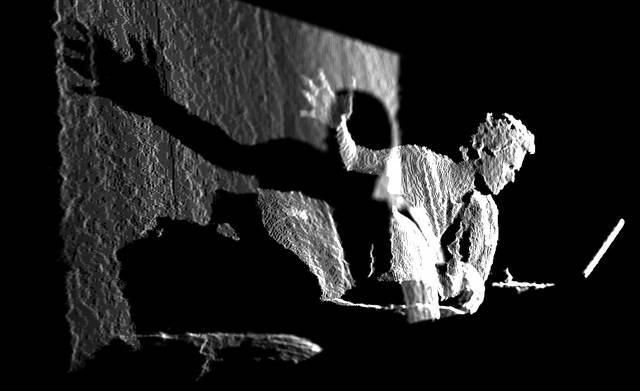
\includegraphics[width=10in]{kyle_kinect.jpg}
\caption{Photo (CC-BY-SA-NC) Kyle McDonald}
\end{figure}

3D range sensors like Velodyne and Kinect generate massive amounts of data, on the order of
{\bf one million data points per second}.

Standard optimization algorithms for real-time perception aren't adequate.

\end{block}

\begin{block}{Related Work: The Registration Problem}

{\bf Iterative Closest Point (ICP) algorithm} 
\begin{figure}
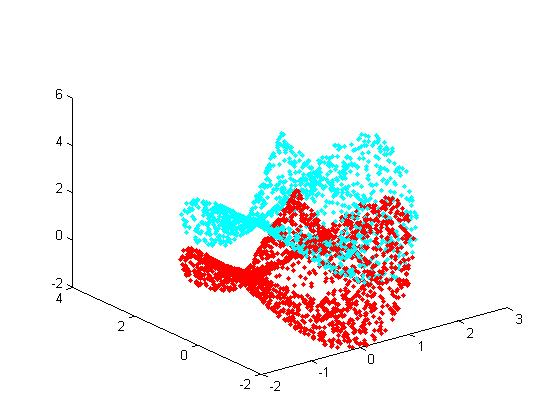
\includegraphics[width=10in]{icpCpp.jpg}
\caption{Photo from Per Bergstr�m via MATLAB FileExchange}
\end{figure}

{\bf Gaussian Mixture Models (GMM)}
\begin{figure}
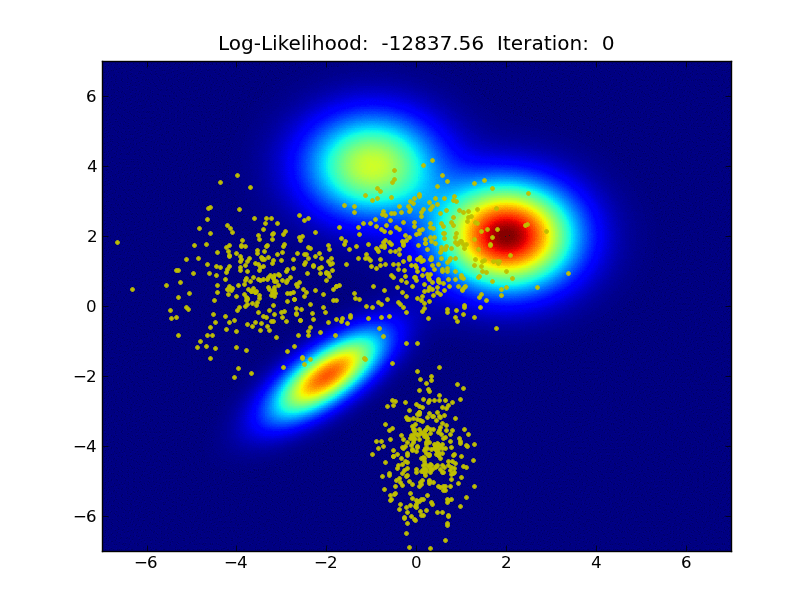
\includegraphics[width=10in]{register2D.png}
\end{figure}

\end{block}
\end{textblock}

\begin{textblock}{27.5}(30.8,5)
\begin{block}{Gaussian Processes (GPs)}
A distribution over functions, fully specified by a mean and a covariance:
$f \sim \mathcal{GP}(m,k)$. Given a set of points $(X,y)$ and a new point $X_*$ for which we want to predict $y_*$, 
distribution is simple: {\bf multivariate Gaussian} with:
$$\mu = K_* (K + \sigma^2 I)^{-1}y$$
$$\Sigma = K_{**} - K_* (K + \sigma^2 I)^{-1} K_*^T$$
\end{block}

\begin{block}{Formulating Registration as an Optimization Problem}
Given a scene and a set of new points, find a rigid transformation $T = [T_x,T_y,T_z,T_s,T_u,T_v,T_w]$ of the new points 
that maximizes their likelihood in the original scene, where the original scene is fit with a GP:
$$min -\ell(T|X,y,X_*,y_*) =$$
$$ \ln|\Sigma| + (T(X_*) - \mu)^T \Sigma^{-1} (T(X_*) - \mu)$$

Note that this problem is not convex---in fact, the minimum we care about may {\bf not} be the global minimum. 
\end{block}
\begin{block}{Gradient Descent}
Partial derivatives must be found with respect to the 7 parameters of $T$. Each can be written in closed form,
using {\bf matrix} and {\bf quaternion} calculus. Numerical stability and speed relies on the {\bf Cholesky} decomposition.
\end{block}

\begin{block}{Experimental Evaluation}
\begin{figure}
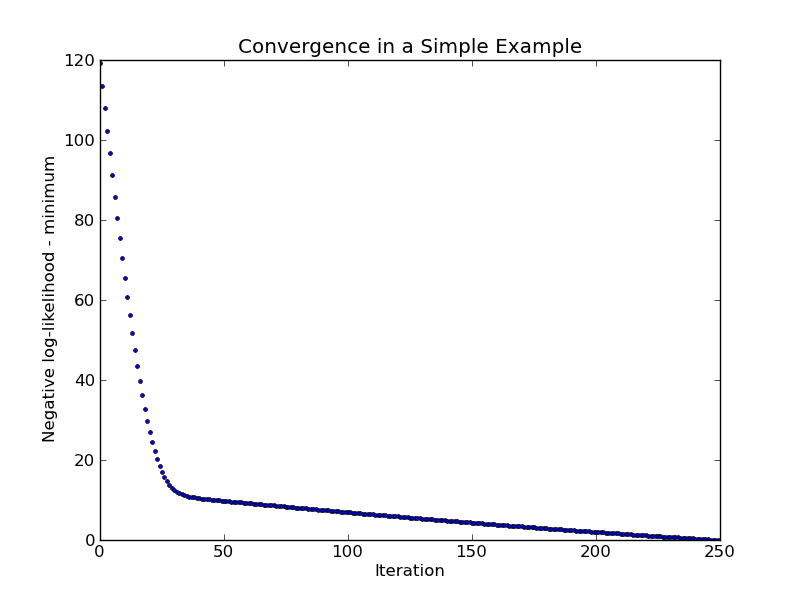
\includegraphics[width=8in]{likelihood.png}
\caption{Convergence}
\end{figure}

\end{block}

\end{textblock}

\begin{textblock}{27}(61,5)

\begin{block}{3D Model}
Dataset: A cloud of 3-D points
Representation: An elevation map (X,Y) $\rightarrow$ Z
The Gaussian Process induces a probability distribution on the elevation of every (X,Y)

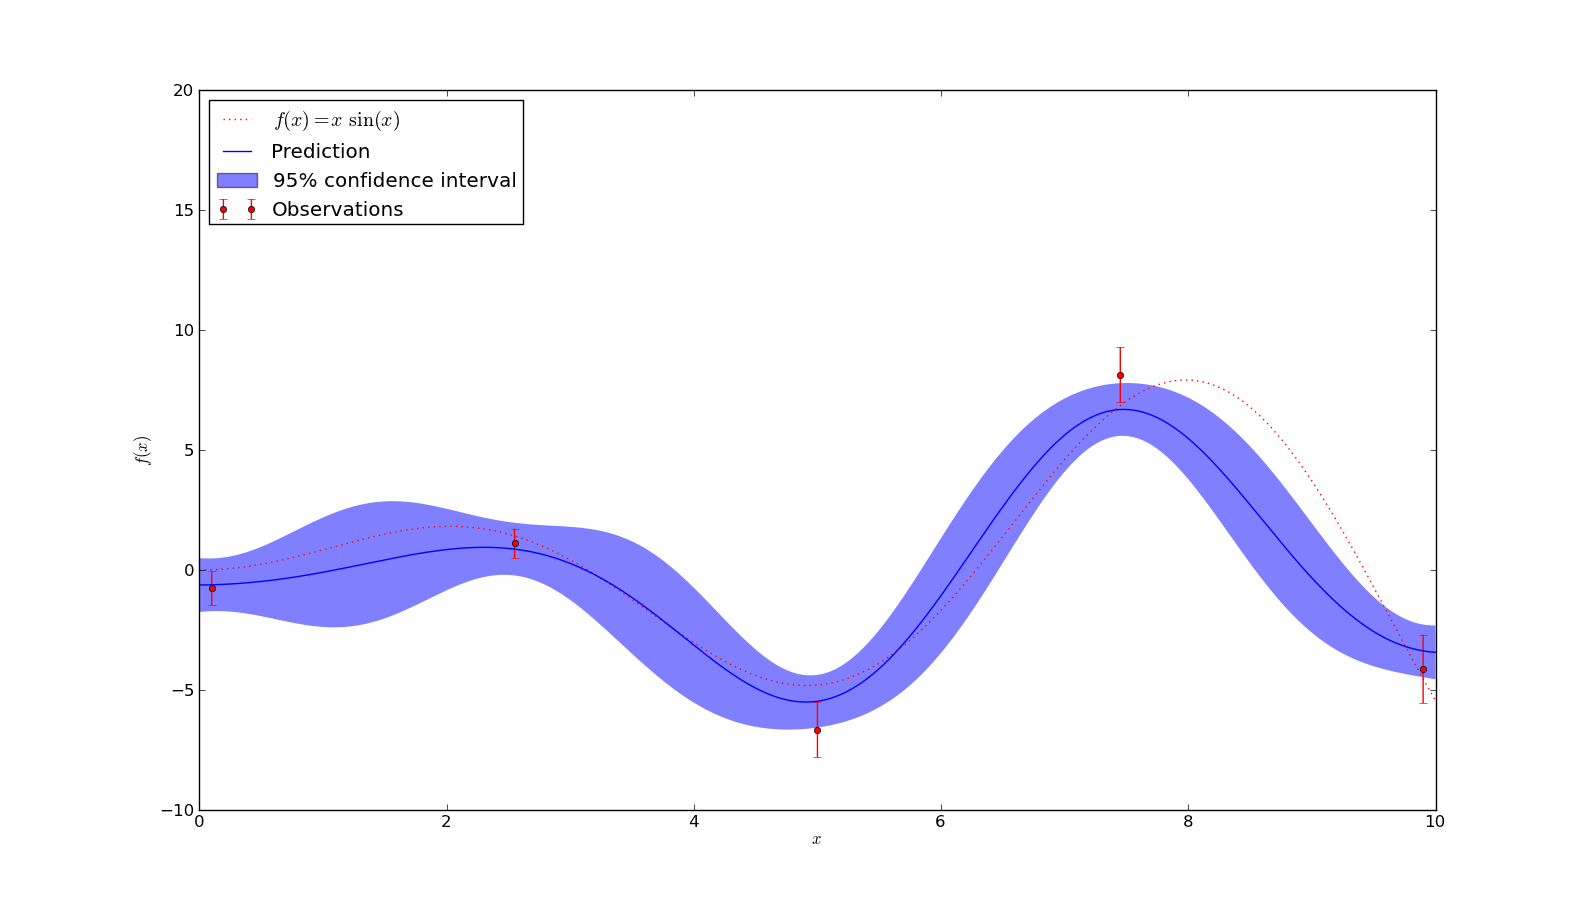
\includegraphics[width=5in]{1DGaussianProcess.png}
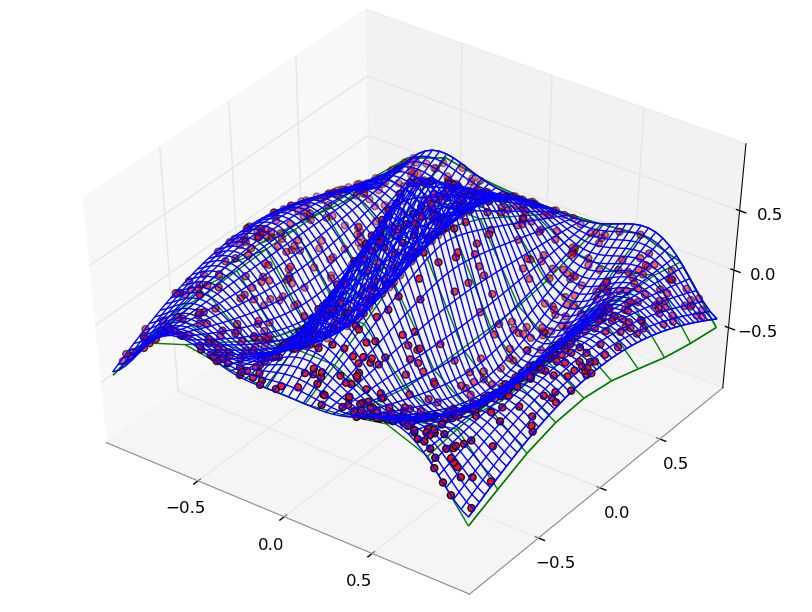
\includegraphics[width=5in]{2DGaussianProcess.png}
\end{block}

\begin{block}{Estimating orientation}
Given two consecutive frames of 3D cloud datasets, we aim to find the most likely rigid transformation that converted the first into the second.

\textbf{Input:} Two consecutive 3D datasets

\textbf{Output:} The most likely rigid transformation from one scene to the other.
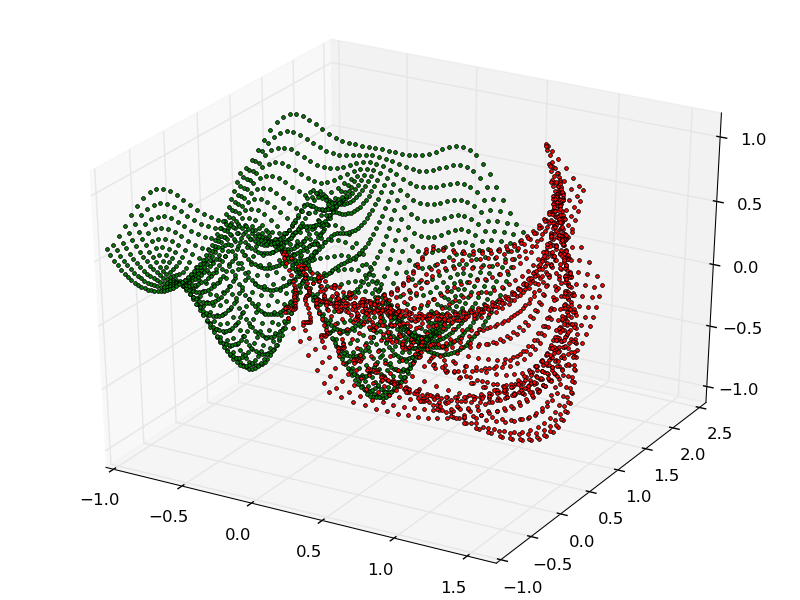
\includegraphics[width=10in]{3DWorldModel.png}
\end{block}

\begin{block}{Experiments}
We generated test data from a smooth distribution with several parameters:
\begin{enumerate}
\item Dataset size (100-2000)
\item Magnitude of transformation between datasets
\end{enumerate}
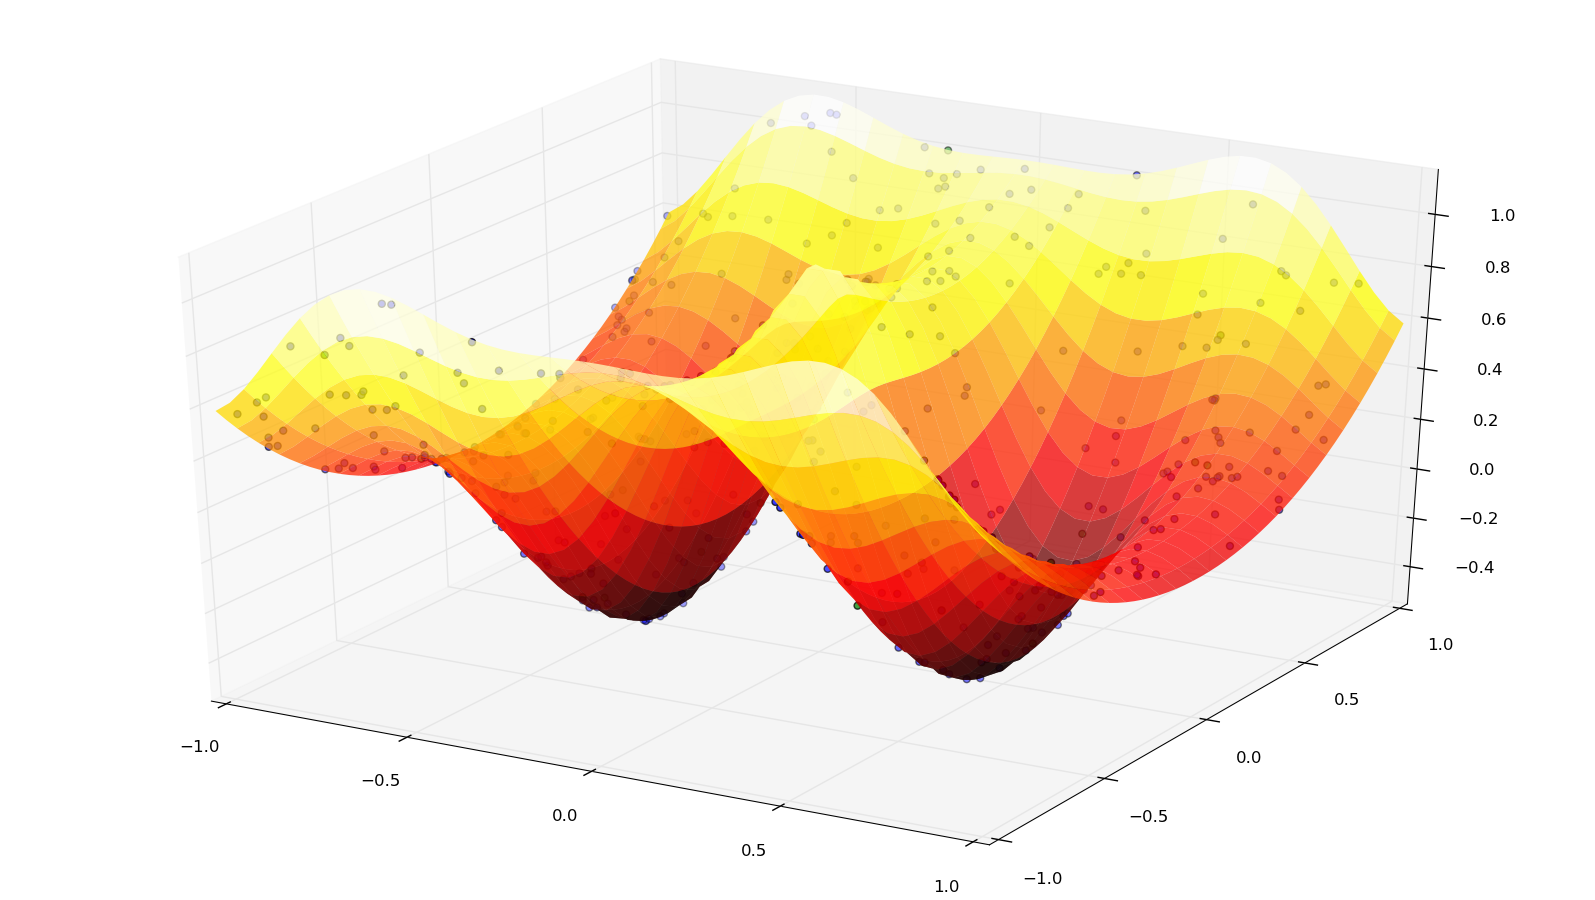
\includegraphics[width=5in]{DistributionPlusPoints.png}
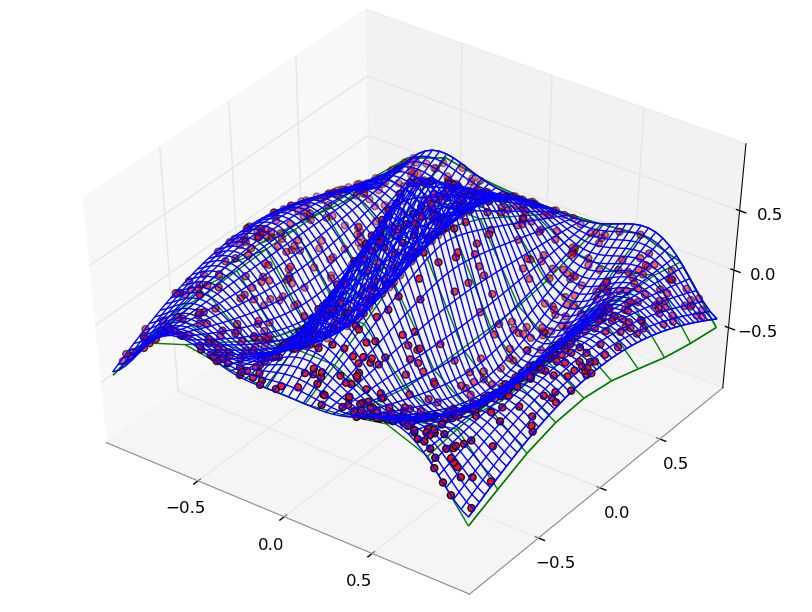
\includegraphics[width=5in]{Reconstruction.png}
\end{block}

\end{textblock}


\begin{textblock}{27}(91,5)

\begin{block}{Parameter space}
Our parameter search space is 7-D ([Tx,Ty,Tz],RotationQuaternion)
A figure of the likelihood space on a 2-D projection of this space follows:
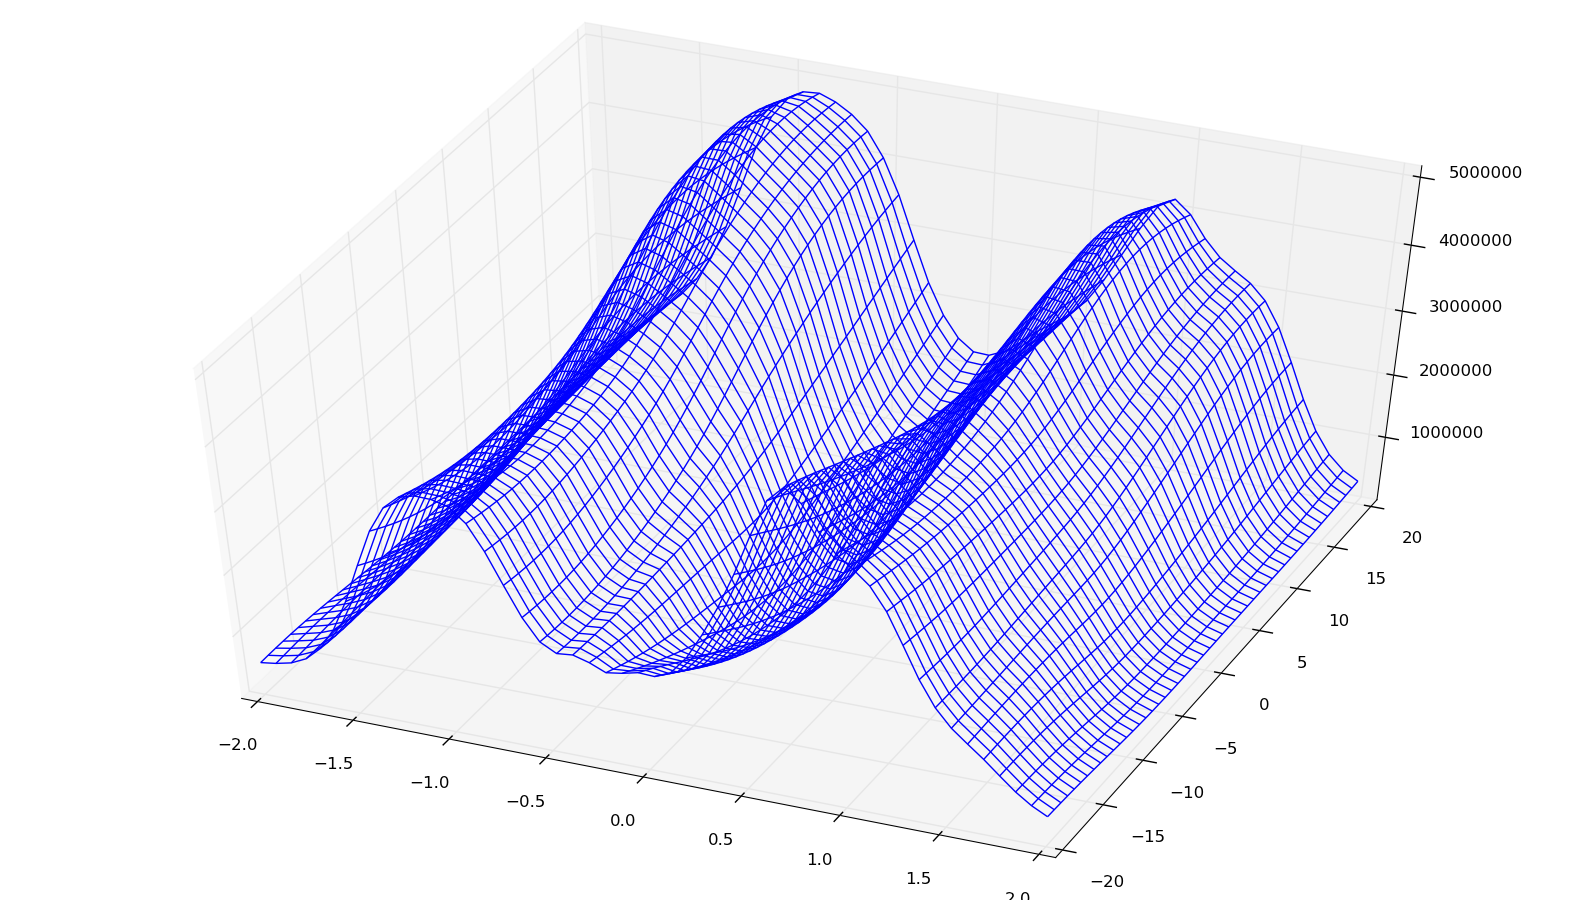
\includegraphics[width=10in]{LLProjection.png}
\end{block}

\begin{block}{Comparison with other methods}
Our method outperforms ICP by x% convergence rate, and is y% faster.

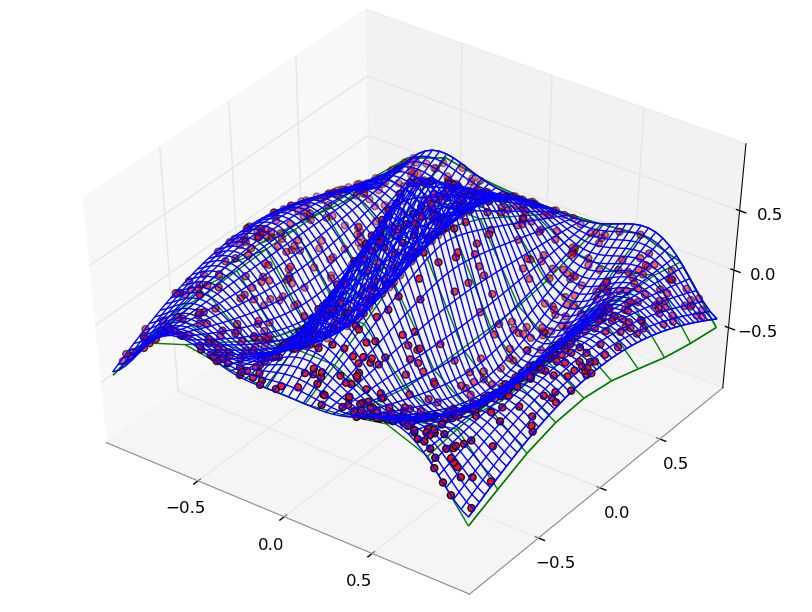
\includegraphics[width=10in]{ConvergenceComparison.png}
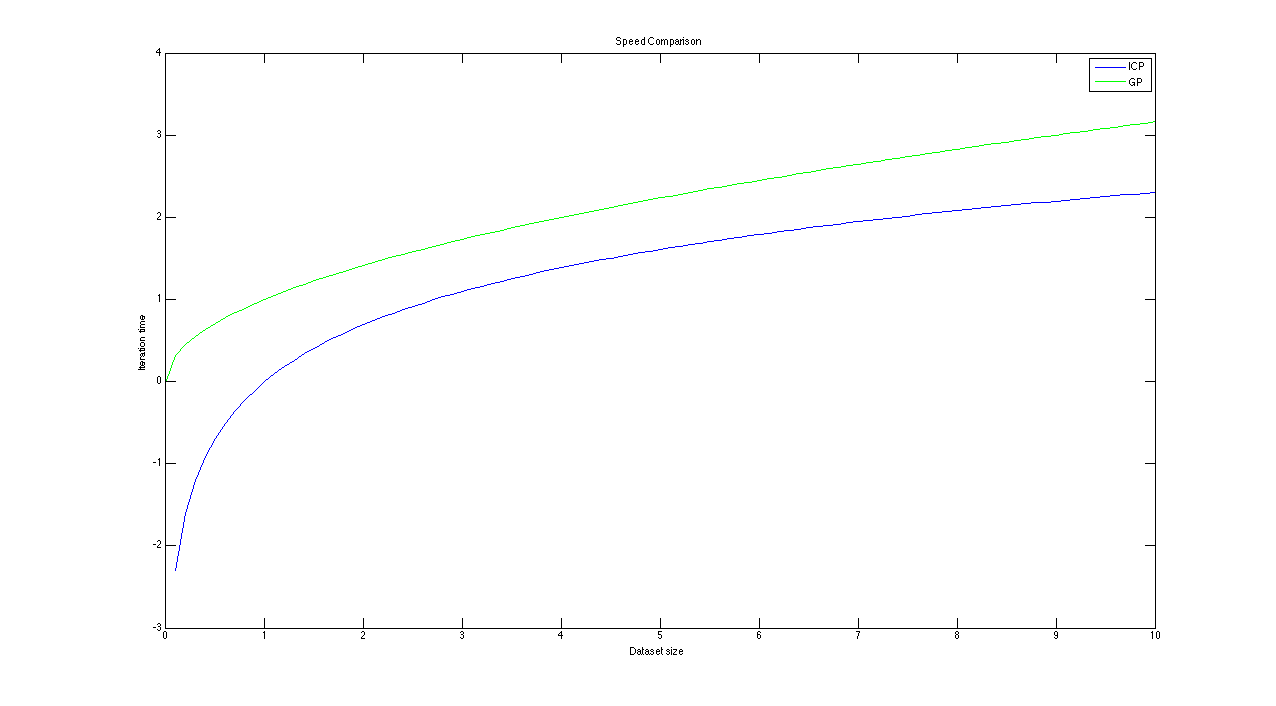
\includegraphics[width=10in]{SpeedComparison.png}
\end{block}

\begin{block}{Conclusions}
\begin{itemize}
\item dunno yet
\item but i'll
\item figure it
\item out
\end{itemize}
\end{block}

\begin{block}{References}
{
 \bibliographystyle{abbrv}
 \bibliography{cmubib}
}
\end{block}

\end{textblock}

\end{frame}
\end{document}
